%%%%%%%%%%%%%%%%%%%%
\subsection{A unified implementation with the reparameterisation trick}

Readers may have noticed that $\mathcal{L}_{\text{VI}}$ has a different form compared to $\mathcal{L}_{\alpha}$ with $\alpha \neq 1$. In this section we show how to unify the implementation for all finite $\alpha$ settings using the \emph{reparameterisation trick} \citep{salimans:reparam2013, kingma:vae2014} as an example. This trick assumes the existence of the mapping $\bm{\theta} = g_{\bm{\phi}}(\bm{\epsilon})$, where the distribution of the noise term $\bm{\epsilon}$ satisfies $q(\bm{\theta}) d\bm{\theta} = p(\bm{\epsilon}) d\bm{\epsilon}$. Then the expectation of a function $F(\bm{\theta})$ over distribution $q(\bm{\theta})$ can be computed as
%
$\mathbb{E}_{q(\bm{\theta})} [F(\bm{\theta})] = \mathbb{E}_{p(\bm{\epsilon})} [F(g_{\bm{\phi}}(\bm{\epsilon}))].$
%
One prevalent example is the Gaussian reparameterisation: $\bm{\theta} \sim \mathcal{N}(\bm{\mu}, \Sigma) \Rightarrow \bm{\theta} = \bm{\mu} + \Sigma^{ \frac{1}{2} } \bm{\epsilon}$, with $\bm{\epsilon} \sim \mathcal{N}(\bm{0}, I)$. 
%
Now we apply the reparameterisation trick to the VR bound
%
\begin{equation}
\mathcal{L}_{\alpha}(q_{\bm{\phi}}; \bm{x}) = \frac{1}{1 - \alpha} \log \mathbb{E}_{\bm{\epsilon}} \left[\left( \frac{p(g_{\bm{\phi}}(\bm{\epsilon}) , \bm{x})}{q(g_{\bm{\phi}}(\bm{\epsilon}))} \right)^{1 - \alpha} \right].
\end{equation}
%
For notational ease we also write $g_{\bm{\phi}} = g_{\bm{\phi}}(\bm{\epsilon})$. Then the gradient of the VR bound w.r.t.~$\bm{\phi}$ (similar for $\bm{\varphi}$) is
\begin{equation}
\begin{aligned}
\nabla_{\bm{\phi}} \mathcal{L}_{\alpha}(q_{\bm{\phi}}; \bm{x}) 
&= \frac{1}{1 - \alpha} \nabla_{\bm{\phi}} \log \mathbb{E}_{\bm{\epsilon}} \left[ \left( \frac{p(g_{\bm{\phi}}, \bm{x})}{q(g_{\bm{\phi}})} \right)^{1 - \alpha} \right] \\
&= \frac{1}{1 - \alpha} \left( \mathbb{E}_{\bm{\epsilon}} \left[ \left( \frac{p(g_{\bm{\phi}}, \bm{x})}{q(g_{\bm{\phi}})} \right)^{1 - \alpha} \right] \right)^{-1} \mathbb{E}_{\bm{\epsilon}} \left[ \nabla_{\bm{\phi}} \left( \frac{p(g_{\bm{\phi}}, \bm{x})}{q(g_{\bm{\phi}})} \right)^{1 - \alpha} \right] \\
&= \frac{1}{1 - \alpha} \left( \mathbb{E}_{\bm{\epsilon}} \left[ \left( \frac{p(g_{\bm{\phi}}, \bm{x})}{q(g_{\bm{\phi}})} \right)^{1 - \alpha} \right] \right)^{-1} \mathbb{E}_{\bm{\epsilon}} \left[ \left( \frac{p(g_{\bm{\phi}}, \bm{x})}{q(g_{\bm{\phi}})} \right)^{1 - \alpha} \nabla_{\bm{\phi}} (1 - \alpha) \log \frac{p(g_{\bm{\phi}}, \bm{x})}{q(g_{\bm{\phi}})} \right] \\
&= \mathbb{E}_{\bm{\epsilon}} \left[ w_{\alpha}(\bm{\epsilon}; \bm{\phi}, \bm{x}) \nabla_{\bm{\phi}} \log \frac{p(g_{\bm{\phi}}, \bm{x})}{q(g_{\bm{\phi}})} \right].
\end{aligned}
\label{eq:chap4_vrbound_gradient_reparam}
\end{equation}
%
where $w_{\alpha}(\bm{\epsilon}; \bm{\phi}, \bm{x}) = \left( \frac{p(g_{\bm{\phi}}(\bm{\epsilon}), \bm{x})}{q(g_{\bm{\phi}}(\bm{\epsilon}))} \right)^{1 - \alpha} \bigg/ \mathbb{E}_{\bm{\epsilon}} \left[ \left( \frac{p(g_{\bm{\phi}}(\bm{\epsilon}), \bm{x})}{q(g_{\bm{\phi}}(\bm{\epsilon}))} \right)^{1 - \alpha} \right]$ denotes the normalised importance weight. 
%
One can show that this recovers the the stochastic gradients of $\mathcal{L}_{\text{VI}}$ by setting $\alpha = 1$ in (\ref{eq:chap4_vrbound_gradient_reparam}) since now $w_{1}(\bm{\epsilon}; \bm{\phi}, \bm{x}) = 1$, which means the resulting algorithm unifies the computation for all finite $\alpha$ settings. For MC approximations, we use $K$ samples to approximately compute the weight $\hat{w}_{\alpha, k}(\bm{\epsilon}_k; \bm{\phi}, \bm{x}) \propto \left( \frac{p(g_{\bm{\phi}}(\bm{\epsilon}_k), \bm{x})}{q(g_{\bm{\phi}}(\bm{\epsilon}_k))} \right)^{1 - \alpha}$, $k = 1, ..., K$, and the stochastic gradient becomes
\begin{equation}
\nabla_{\bm{\phi}} \hat{\mathcal{L}}_{\alpha, K}(q_{\bm{\phi}}; \bm{x}) 
= \sum_{k=1}^K \left[ \hat{w}_{\alpha, k}(\bm{\epsilon}_k; \bm{\phi}, \bm{x}) \nabla_{\bm{\phi}} \log \frac{p(g_{\bm{\phi}}(\bm{\epsilon}_k), \bm{x})}{q(g_{\bm{\phi}}(\bm{\epsilon}_k))} \right].
\end{equation}
When $\alpha = 1$, $\hat{w}_{1, k}(\bm{\epsilon}_k; \bm{\phi}, \bm{x}) = 1/K$, and it recovers the stochastic gradient VI method \citep{kingma:vae2014}.

To speed-up learning \citet{burda:iwae2016} suggested back-propagating only one sample $\bm{\epsilon}_j$ with $j \sim p_j = \hat{w}_{\alpha, j}$, which can be easily extended to our framework. Importantly, the use of different $\alpha < 1$ indicates the degree of emphasis placed upon locations where the approximation $q$ under-estimates $p$, and in the extreme case $\alpha \rightarrow -\infty$, the algorithm chooses the sample that has the \emph{maximum} unnormalised importance weight. 
%
We name this approach \emph{VR-max} and summarise it and the general case in Algorithm \ref{alg:vr_max}. 
%
Note that VR-max (and VR-$\alpha$ with $\alpha < 0$ and MC approximations) does \emph{not} minimise $\mathrm{D}_{1-\alpha}^{R}[p||q]$. It is true that $\mathcal{L}_{\alpha} \geq \log p(\bm{x})$ for negative $\alpha$ values. However Corollary \ref{thm:chap4_vrbound_alpha_k_existence} suggests that the tightest MC approximation for given $K$ has non-positive $\alpha_K$ value, or might not even exist. Furthermore the optimal $\alpha_K$ value becomes more negative as the mismatch between $q$ and $p$ increases, e.g.~the VAE uses a uni-modal $q$ distribution to approximate the typically multi-modal exact posterior.



\begin{figure}[!t]
% UGLY USE OF \vspace & \hspace follows
\begin{minipage}[b]{0.55\linewidth}
\centering
\begin{algorithm}[H] 
\caption{One gradient step for VR-$\alpha$/VR-max with single backward pass. Here $\hat{w}(\bm{\epsilon}_k; \bm{x})$ short-hands $\hat{w}_{0, k}(\bm{\epsilon}_k; \bm{\phi}, \bm{x})$ in the main text.} \small
\label{alg:vr_max} 
\begin{algorithmic}[1] 
	\STATE given the current datapoint $\bm{x}$, sample \\$\bm{\epsilon}_1, ..., \bm{\epsilon}_K \sim p(\bm{\epsilon})$
	\STATE for $k = 1, ..., K$, compute the unnormalised weight \\
	$\log \hat{w}(\bm{\epsilon}_k; \bm{x}) = \log p(g_{\bm{\phi}}(\bm{\epsilon}_k), \bm{x}) - \log q(g_{\bm{\phi}}(\bm{\epsilon}_k)|\bm{x})$
	\STATE choose the sample $\bm{\epsilon}_{j}$ to back-propagate: \\
	if $|\alpha| < \infty$: $j \sim p_k$ where $p_k \propto \hat{w}(\bm{\epsilon}_k; \bm{x})^{1 - \alpha}$ \\
	if $\alpha = -\infty$: $j = \argmax_{k} \log \hat{w}(\bm{\epsilon}_k; \bm{x})$ 
	\STATE return the gradients $\nabla_{\bm{\phi}} \log \hat{w}(\bm{\epsilon}_{j}; \bm{x})$
\end{algorithmic}
\end{algorithm}
\end{minipage}
%
\hfill
\begin{minipage}[b]{0.4\linewidth}
\centering
 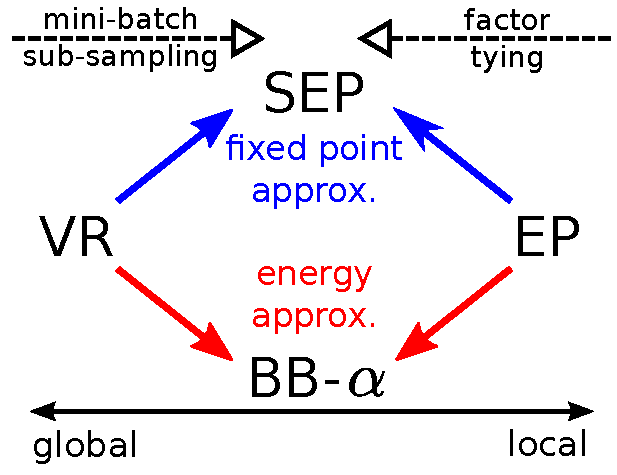
\includegraphics[width=0.9\linewidth]{vr_ep_relationship.pdf} 
 \vspace{-0.1in}
 \captionof{figure}{Connecting local and global divergence minimisation.}
 \label{fig:vr_ep_relationship}
\end{minipage}
%\quad
%
\end{figure}

